% 2008 年湖北卷理科第 19 题：以 O 为圆心、|AB|=4 为直径的半圆 ADB，OD ⊥ AB，P 在半圆弧上，
%   ∠POB=30°。
% 来源 PDF：gaokaomath-src/普通高考/2008/2008湖北理.pdf
% SHA-256：54077e9ac5227f015a8972bfc4c4415b503b31acdf0a6e7cd51782afa098a112
% 原页：2008湖北理.pdf 第 2 页（A3 三栏）第 1 栏，书页码 450。
% 绘制依据：按原页画上半圆（圆心 O、半径 2），AB 水平、D 在最高点，P 位于 B 一侧 30° 处并连 OP。
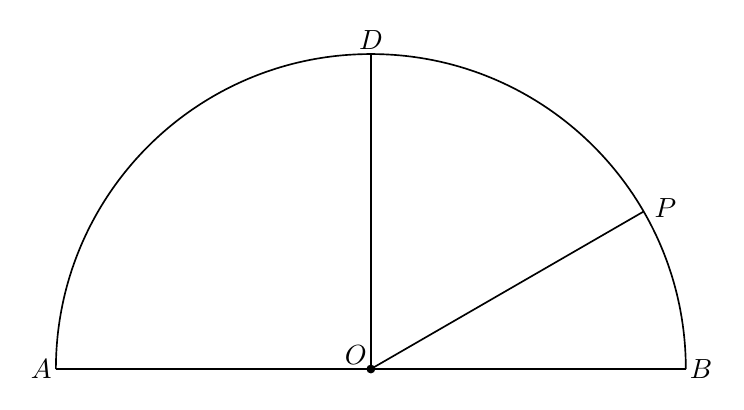
\begin{tikzpicture}[scale=2.0, semithick, every node/.style={inner sep=1.2pt}]
  % 半圆弧（上半）
  \draw (2,0) arc[start angle=0, end angle=180, radius=2];

  % 直径 AB 与半径 OD、OP
  \draw (-2,0) -- (2,0);
  \draw (0,0) -- (0,2);
  \draw (0,0) -- (30:2);

  \fill (0,0) circle (0.8pt);

  \node[left] at (-2,0) {$A$};
  \node[right] at (2,0) {$B$};
  \node[above] at (0,2) {$D$};
  \node[above left] at (0,0) {$O$};
  \node[right] at (30:2.05) {$P$};
\end{tikzpicture}
